A continuación se presentan las instrucciones de instalación de \textbf{oFlute}
en sistemas GNU/Linux basados en paquetería Debian\cite{refdebian}, por
ser los que más auge están teniendo en la actualidad. Tomaremos como referencia
la distribución Ubuntu 10.10 Maverick\cite{refubuntu}.

\section{Instalación de dependencias}

El primer paso a la hora de instalar oFlute es hacernos con las dependencias del
proyecto. Para ello, utilizaremos el gestor \texttt{apt-get}, pero para otros
sistemas el procedimiento será similar.

Primero, instalaremos las dependencias de la biblioteca Gosu:

\begin{minted}{bash}
  sudo apt-get install g++ libgl1-mesa-dev libpango1.0-dev \
  libopenal-dev libsndfile-dev libxdamage-dev libsdl-ttf2.0-dev \
  libboost-dev libfreeimage3 libfreeimage-dev
\end{minted}

Seguidamente, instalaremos el resto de dependencias:

\begin{minted}{bash}
  sudo apt-get install libboost-regex-dev libboost-filesystem-dev \ 
  libboost-thread-dev libpulse-dev
\end{minted}

\section{Descarga del código fuente}

El siguiente paso será hacernos con una copia local del repositorio, que
contiene el código fuente. Al tratarse de un proyecto libre, el repositorio es
de acceso público\cite{ofluteforja}.

Haciendo uso del comando \texttt{svn}, haremos una copia local del repositorio
Subversion\cite{refsubversion} en nuestro sistema con la siguiente orden:

\begin{minted}{bash}
  svn checkout http://oflute.googlecode.com/svn/trunk oflute
\end{minted}

Con ello, se creará una carpeta llamada \texttt{oflute} en la que se encontrarán
los ficheros de la rama principal (\texttt{trunk}) del proyecto.

\section{Compilación}

Como se ha comentado previamente, será necesario compilar la biblioteca Gosu
previamente. Para ello, se ha facilitado un objetivo en el script de compilación
\texttt{Makefile}~\cite{refmakefile} que automatiza el proceso.

Así, el primer paso será, estando en la carpeta recién creada, utilizar el
siguiente comando:

\begin{minted}{bash}
  make libgosu
\end{minted}

Una vez concluida la compilación de Gosu, pasaremos a compilar el propio
proyecto mediante la siguiente orden:

\begin{minted}{bash}
  make
\end{minted}

\section{Configuración del micrófono}
Antes de poder lanzar el juego, será necesario configurar las opciones de audio
del sistema operativo. Por defecto, la entrada de audio suele estar mutada, por
lo que será imposible que la aplicación tenga acceso al sonido proveniente del
micrófono.

Siguiendo con la referencia de Ubuntu, iremos al menú \textit{Sistema}, luego a
\textit{Preferencias} y, finalmente, elegiremos \textit{Sonido}. Una vez ahí,
pasaremos a la pestaña \textit{Entrada} y, en caso de que estuviera marcada,
desmarcaremos la opción \textit{Silenciar}, tal y como muestra la imagen.

\begin{figure}[h!]
  \centering
  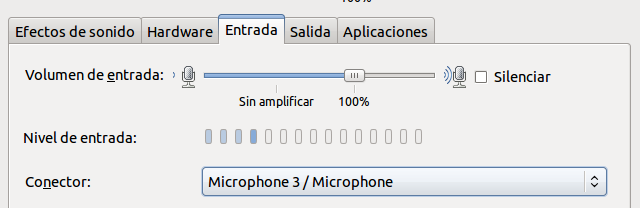
\includegraphics[width=0.75\textwidth]{apendice_manual_instalacion/imagen_captura_1}
  \caption{Panel de configuración del micrófono}
\end{figure}

\vspace{-1cm}

\section{Ejecución}

Al término de las anteriores etapas, se habrá generado un ejecutable de nombre
\texttt{oflute}, por lo que será posible lanzar la aplicación a través del
siguiente comando:

\begin{minted}{bash}
  ./oflute
\end{minted}

%%% Local Variables: 
%%% mode: latex
%%% TeX-master: "../memoria"
%%% End: 
